% 书末「其它你可能会喜欢的书籍」（原书 printed 414–416 / pdf 427–429）
% 首页：30bp 右对齐标题 baseline 104.9；引言 144.4；封面图 96.8×119.3 (top 155.7)；
%      书名 Palatino-Bold 12 baseline 295.7；作者 310.1；ISBN 333.5；
%      要点基线 355.6 起，节距 14.75；符号 x 95.6，正文 x 104.7
% 续页：页眉左斜体“其它你可能会喜欢的书籍”，页脚 [页码]
\thispagestyle{empty}
\markboth{}{}
\begingroup
\parindent 0bp
\parskip 0bp
\vspace*{-33.9bp}%
\noindent 如果你喜欢这本书，可能也会对 Packt 出版的这些其他书籍感兴趣：\par
\vspace{8.2bp}
\noindent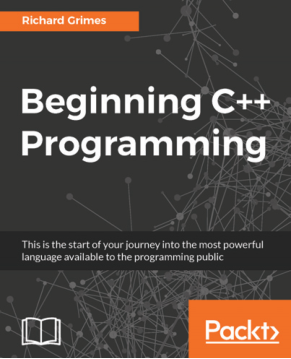
\includegraphics[width=96.8bp,height=119.3bp]{images/p427_i02.png}\par
\vspace{6.3bp}
{\rmfamily\bfseries\fontsize{12bp}{14.4bp}\selectfont Beginning C++ Programming\par}
\vspace{0bp}
{\rmfamily\fontsize{12bp}{14.4bp}\selectfont Richard Grimes\par}
\vspace{9.0bp}
{\rmfamily\fontsize{12bp}{14.4bp}\selectfont ISBN：978-1-78712-494-3\par}
\vspace{9.5bp}
{\fontsize{10.5bp}{12.6bp}\selectfont
\noindent\hangindent 48bp\hangafter 1\hspace*{38.9bp}\textbullet\hspace{5.4bp}%
熟悉 C++ 项目的结构\par
\vspace{2.15bp}
\noindent\hangindent 48bp\hangafter 1\hspace*{38.9bp}\textbullet\hspace{5.4bp}%
识别语言中的主要结构：函数与类\par
\vspace{2.15bp}
\noindent\hangindent 48bp\hangafter 1\hspace*{38.9bp}\textbullet\hspace{5.4bp}%
自信地找出代码的执行流程\par
\vspace{2.15bp}
\noindent\hangindent 48bp\hangafter 1\hspace*{38.9bp}\textbullet\hspace{5.4bp}%
了解标准库提供的各种功能\par
\vspace{2.15bp}
\noindent\hangindent 48bp\hangafter 1\hspace*{38.9bp}\textbullet\hspace{5.4bp}%
深入理解面向对象的基本概念\par
\vspace{2.15bp}
\noindent\hangindent 48bp\hangafter 1\hspace*{38.9bp}\textbullet\hspace{5.4bp}%
学会调试自己的程序\par
\vspace{2.15bp}
\noindent\hangindent 48bp\hangafter 1\hspace*{38.9bp}\textbullet\hspace{5.4bp}%
熟悉标准 C++ 库\par}
\endgroup

% ---- 第 2 页：Modern C++ Programming Cookbook（续页有页眉页脚）----
\clearpage
\markboth{其他你可能会喜欢的书籍}{}
\begingroup
\parindent 0bp
\parskip 0bp
\vspace*{-11.7bp}%
\noindent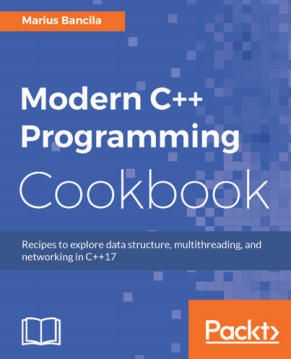
\includegraphics[width=96.8bp,height=119.3bp]{images/p428_i02.png}\par
\vspace{1.7bp}
{\rmfamily\bfseries\fontsize{12bp}{14.4bp}\selectfont Modern C++ Programming Cookbook\par}
\vspace{-2.9bp}
{\rmfamily\fontsize{12bp}{14.4bp}\selectfont Marius Bancila\par}
\vspace{8.2bp}
{\rmfamily\fontsize{12bp}{14.4bp}\selectfont ISBN：978-1-78646-518-4\par}
\vspace{10.9bp}
{\fontsize{10.5bp}{12.6bp}\selectfont
\noindent\hangindent 48bp\hangafter 1\hspace*{38.9bp}\textbullet\hspace{5.4bp}%
了解新的核心语言特性以及它们旨在解决的问题\par
\vspace{2.15bp}
\noindent\hangindent 48bp\hangafter 1\hspace*{38.9bp}\textbullet\hspace{5.4bp}%
理解对线程与并发的标准支持，并了解如何把它们用于日常的基础任务\par
\vspace{2.15bp}
\noindent\hangindent 48bp\hangafter 1\hspace*{38.9bp}\textbullet\hspace{5.4bp}%
利用 C++ 的特性提升健壮性与性能\par
\vspace{2.15bp}
\noindent\hangindent 48bp\hangafter 1\hspace*{38.9bp}\textbullet\hspace{5.4bp}%
探索广泛使用的 C++ 测试框架，并实现各种有用的模式与惯用法\par
\vspace{2.15bp}
\noindent\hangindent 48bp\hangafter 1\hspace*{38.9bp}\textbullet\hspace{5.4bp}%
处理各种类型的字符串，并考察编译的各个方面\par
\vspace{2.15bp}
\noindent\hangindent 48bp\hangafter 1\hspace*{38.9bp}\textbullet\hspace{5.4bp}%
探索函数与可调用对象，重点关注现代特性\par
\vspace{2.15bp}
\noindent\hangindent 48bp\hangafter 1\hspace*{38.9bp}\textbullet\hspace{5.4bp}%
使用标准库，配合容器、算法与迭代器工作\par
\vspace{2.15bp}
\noindent\hangindent 48bp\hangafter 1\hspace*{38.9bp}\textbullet\hspace{5.4bp}%
使用正则表达式进行查找与替换字符串操作\par
\vspace{2.15bp}
\noindent\hangindent 48bp\hangafter 1\hspace*{38.9bp}\textbullet\hspace{5.4bp}%
利用新的文件系统库处理文件与目录\par
\vspace{2.15bp}
\noindent\hangindent 48bp\hangafter 1\hspace*{38.9bp}\textbullet\hspace{5.4bp}%
使用标准库新增的工具解决开发者遇到的常见问题，包括 string\_view、any、optional 与 variant 类型\par}
\endgroup

% ---- 第 3 页：留一篇书评 ----
\clearpage
\markboth{其他你可能会喜欢的书籍}{}
\begingroup
\parindent 0bp
\parskip 0bp
\vspace*{-15.7bp}%
{\sffamily\bfseries\fontsize{20bp}{24bp}\selectfont 留一篇书评 —— 让其他读者了解你的看法\par}
\vspace{29.6bp}
{\fontsize{10.5bp}{12.6bp}\selectfont
\noindent 请在你购买本书的站点上留下书评，把你的想法分享给其他人。如果你是在 Amazon 购买的本书，请在这本书的 Amazon 页面上给我们留下真诚的评论。这样做很重要，其他潜在读者可以看到并使用你的客观意见做出购买决策，我们也可以了解客户对我们产品的看法，我们的作者同样能看到他们与 Packt 合作创作的这本书的反馈。这只会占用你几分钟时间，却对其他潜在客户、我们的作者和 Packt 都很有价值。谢谢！\par}
\endgroup
